\PassOptionsToPackage{unicode=true}{hyperref} % options for packages loaded elsewhere
\PassOptionsToPackage{hyphens}{url}
%
\documentclass[ignorenonframetext,]{beamer}
\usepackage{pgfpages}
\setbeamertemplate{caption}[numbered]
\setbeamertemplate{caption label separator}{: }
\setbeamercolor{caption name}{fg=normal text.fg}
\beamertemplatenavigationsymbolsempty
% Prevent slide breaks in the middle of a paragraph:
\widowpenalties 1 10000
\raggedbottom
\setbeamertemplate{part page}{
\centering
\begin{beamercolorbox}[sep=16pt,center]{part title}
  \usebeamerfont{part title}\insertpart\par
\end{beamercolorbox}
}
\setbeamertemplate{section page}{
\centering
\begin{beamercolorbox}[sep=12pt,center]{part title}
  \usebeamerfont{section title}\insertsection\par
\end{beamercolorbox}
}
\setbeamertemplate{subsection page}{
\centering
\begin{beamercolorbox}[sep=8pt,center]{part title}
  \usebeamerfont{subsection title}\insertsubsection\par
\end{beamercolorbox}
}
\AtBeginPart{
  \frame{\partpage}
}
\AtBeginSection{
  \ifbibliography
  \else
    \frame{\sectionpage}
  \fi
}
\AtBeginSubsection{
  \frame{\subsectionpage}
}
\usepackage{lmodern}
\usepackage{amssymb,amsmath}
\usepackage{ifxetex,ifluatex}
\usepackage{fixltx2e} % provides \textsubscript
\ifnum 0\ifxetex 1\fi\ifluatex 1\fi=0 % if pdftex
  \usepackage[T1]{fontenc}
  \usepackage[utf8]{inputenc}
  \usepackage{textcomp} % provides euro and other symbols
\else % if luatex or xelatex
  \usepackage{unicode-math}
  \defaultfontfeatures{Ligatures=TeX,Scale=MatchLowercase}
\fi
% use upquote if available, for straight quotes in verbatim environments
\IfFileExists{upquote.sty}{\usepackage{upquote}}{}
% use microtype if available
\IfFileExists{microtype.sty}{%
\usepackage[]{microtype}
\UseMicrotypeSet[protrusion]{basicmath} % disable protrusion for tt fonts
}{}
\IfFileExists{parskip.sty}{%
\usepackage{parskip}
}{% else
\setlength{\parindent}{0pt}
\setlength{\parskip}{6pt plus 2pt minus 1pt}
}
\usepackage{hyperref}
\hypersetup{
            pdftitle={DDP\_ReproduciblePitch},
            pdfauthor={Luisiana Sabbatini},
            pdfborder={0 0 0},
            breaklinks=true}
\urlstyle{same}  % don't use monospace font for urls
\newif\ifbibliography
\usepackage{graphicx,grffile}
\makeatletter
\def\maxwidth{\ifdim\Gin@nat@width>\linewidth\linewidth\else\Gin@nat@width\fi}
\def\maxheight{\ifdim\Gin@nat@height>\textheight\textheight\else\Gin@nat@height\fi}
\makeatother
% Scale images if necessary, so that they will not overflow the page
% margins by default, and it is still possible to overwrite the defaults
% using explicit options in \includegraphics[width, height, ...]{}
\setkeys{Gin}{width=\maxwidth,height=\maxheight,keepaspectratio}
\setlength{\emergencystretch}{3em}  % prevent overfull lines
\providecommand{\tightlist}{%
  \setlength{\itemsep}{0pt}\setlength{\parskip}{0pt}}
\setcounter{secnumdepth}{0}

% set default figure placement to htbp
\makeatletter
\def\fps@figure{htbp}
\makeatother


\title{DDP\_ReproduciblePitch}
\author{Luisiana Sabbatini}
\date{7/10/2020}

\begin{document}
\frame{\titlepage}

\begin{frame}{Reproducible Pitch Presentation}
\protect\hypertarget{reproducible-pitch-presentation}{}

This Application uses data about motor trend car road test dataset, To
demonstrate various capabilities from the Developing Data Products
Course. The Application provides visualization about cars' miles per
gallon performance.

Using Shiny UI Server Application.

Adding customization to the plot. One Input Widget (Slide Bar). Using
Reactive function. Shiny Application Link :
\url{https://omersect.shinyapps.io/project/} Github Repository Link :
\url{https://github.com/omershect/Course-Project-Shiny-Application-and-Reproducible-Pitch}

\end{frame}

\begin{frame}{The Data}
\protect\hypertarget{the-data}{}

The data was extracted from the 1974 Motor Trend US magazine, and
comprises fuel consumption and 10 aspects of automobile design and
performance for 32 automobiles (1973--74 models).

It is a data frame with 32 observations on 11 (numeric) variables.

{[}, 1{]} mpg Miles/(US) gallon {[}, 2{]} cyl Number of cylinders {[},
3{]} disp Displacement (cu.in.) {[}, 4{]} hp Gross horsepower {[}, 5{]}
drat Rear axle ratio {[}, 6{]} wt Weight (1000 lbs) {[}, 7{]} qsec 1/4
mile time {[}, 8{]} vs Engine (0 = V-shaped, 1 = straight) {[}, 9{]} am
Transmission (0 = automatic, 1 = manual) {[},10{]} gear Number of
forward gears {[},11{]} carb Number of carburetors

\end{frame}

\begin{frame}{The Application Functionality}
\protect\hypertarget{the-application-functionality}{}

You can select the variable you wish to plot

You can slide the number of bins for the histogram plotted

\end{frame}

\begin{frame}{Application User Interface}
\protect\hypertarget{application-user-interface}{}

\begin{figure}
\centering
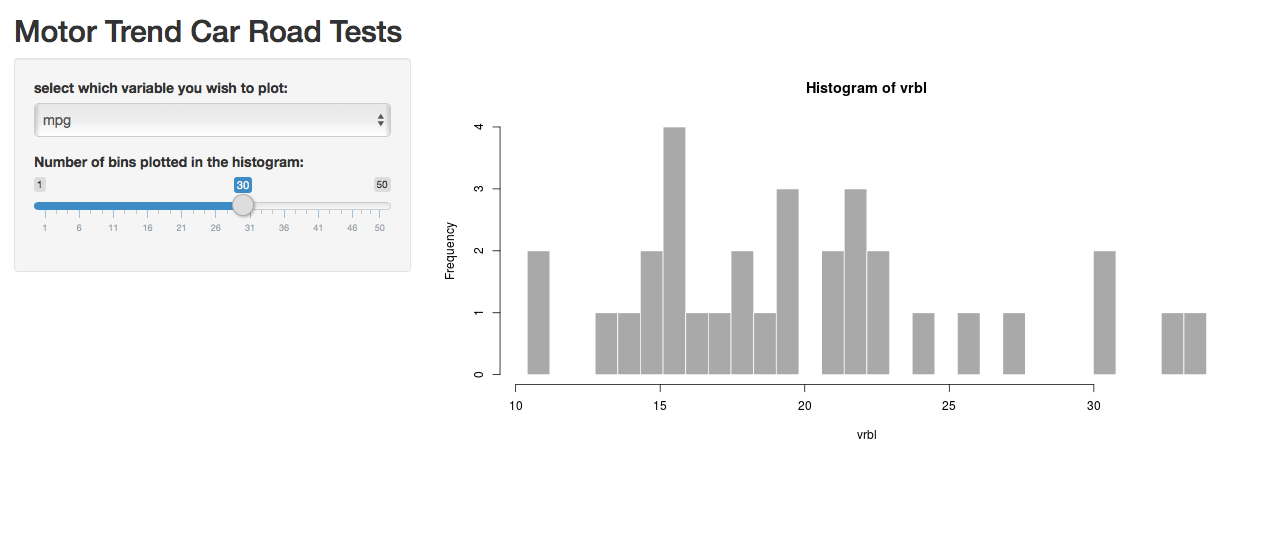
\includegraphics{AppUI.png}
\caption{main page of the application}
\end{figure}

\end{frame}

\end{document}
